\documentclass[12pt,a4paper]{article}
\usepackage[utf8]{inputenc}
\usepackage[french]{babel}
\usepackage[T1]{fontenc}
\usepackage{amsmath}
\usepackage{amsfonts}
\usepackage{amssymb}
\usepackage{graphicx}
\usepackage[left=2cm,right=2cm,top=3cm,bottom=2cm]{geometry}
\usepackage{multicol}
\usepackage[thinspace,thinqspace,amssymb]{SIunits}
\usepackage{pifont}
\usepackage{tikz}
\usepackage{multicol}
\usepackage{fourier}
\usepackage{setspace}
\usepackage{enumitem}

\usepackage{url}
\usepackage[breaklinks]{hyperref}
\hypersetup{
    colorlinks=true,
    linkcolor=red_f,
    citecolor=bleu_f,
    filecolor=green_f,
    urlcolor=bleu_f
}
\usepackage[hyphenbreaks]{breakurl}

\renewcommand{\familydefault}{\sfdefault}

\usepackage{xcolor}
\definecolor{gray_f}{RGB}{68,84,106}
\definecolor{gray_c}{RGB}{214,220,229}
\definecolor{bleu_f}{RGB}{91,155,213}
\definecolor{bleu_c}{RGB}{222,235,247}
\definecolor{red_f}{RGB}{204,0,0}
\definecolor{red_c}{RGB}{245,204,204}
\definecolor{orange_f}{RGB}{237,125,49}
\definecolor{orange_c}{RGB}{251,229,214}
\definecolor{green_f}{RGB}{112,173,71}
\definecolor{green_c}{RGB}{226,240,217}
\definecolor{yellow_f}{RGB}{255,192,0}
\definecolor{yellow_c}{RGB}{255,242,204}

\usepackage{fancyhdr}
\pagestyle{fancy}
\lhead{\textcolor{gray_f}{Physique-Chimie\\R. METZDORFF}}
\chead{\textcolor{gray_f}{Lycée Suzanne Valadon}}
\rhead{\textcolor{gray_f}{2020-2021}}
\renewcommand{\headrulewidth}{0.4pt}
\let\HeadRule\headrule
\renewcommand\headrule{\color{gray_f}\HeadRule}

%%%%% New environnements
\usepackage[framemethod=tikz]{mdframed}
\usepackage{chngcntr}

%%% header
\mdfdefinestyle{s_head}{%
	linecolor=gray_f!,
	outerlinewidth=3pt,%
	frametitlerule=false,
	topline=false,
	bottomline=false,
	rightline=false,
	leftline=false,
	backgroundcolor=gray_c,
	innertopmargin=8pt,
	roundcorner=0pt,
	nobreak=true,
	fontcolor=gray_f
}
\newmdenv[style=s_head]{header_env}
\newenvironment{header}
{%\stepcounter{exa}%
	\addcontentsline{ldf}{figure}{0}%
	\begin{header_env}\centering\LARGE\bf}
	{\end{header_env}}
	
%%% definition
\mdfdefinestyle{s_def}{%
	linecolor=red_f!,
	outerlinewidth=3pt,%
	frametitlerule=false,
	topline=false,
	bottomline=false,
	rightline=false,
	leftline=true,
	backgroundcolor=red_c,
	innertopmargin=8pt,
	roundcorner=0pt,
	nobreak=true,
	fontcolor=red_f
}
\newmdenv[style=s_def]{def_env}
\newenvironment{definition}
{%\stepcounter{exa}%
	\addcontentsline{ldf}{figure}{0}%
	\begin{def_env}\textbf{Définition :}}
	{\end{def_env}}

%%% exemple
\mdfdefinestyle{s_ex}{%
	linecolor=gray_f!,
	outerlinewidth=3pt,%
	frametitlerule=false,
	topline=false,
	bottomline=false,
	rightline=false,
	leftline=true,
	backgroundcolor=gray_c,
	innertopmargin=8pt,
	roundcorner=0pt,
	nobreak=true,
	fontcolor=gray_f
}
\newmdenv[style=s_ex]{ex_env}
\newenvironment{exemple}
{%\stepcounter{exa}%
	\addcontentsline{ldf}{figure}{0}%
	\begin{ex_env}\textbf{Exemple :}}
	{\end{ex_env}}

%%% analyse a priori
\mdfdefinestyle{s_prior}{%
	linecolor=green_f!,
	outerlinewidth=3pt,%
	frametitlerule=false,
	topline=false,
	bottomline=false,
	rightline=false,
	leftline=true,
	backgroundcolor=green_c,
	innertopmargin=8pt,
	roundcorner=0pt,
	nobreak=true,
	fontcolor=green_f
}
\newmdenv[style=s_prior]{prior_env}
\newenvironment{prior}
{%\stepcounter{exa}%
	\addcontentsline{ldf}{figure}{0}%
	\begin{prior_env}\textbf{A priori :}}
	{\end{prior_env}}

%%% analyse a posteriori
\mdfdefinestyle{s_post}{%
	linecolor=green_f!,
	outerlinewidth=3pt,%
	frametitlerule=false,
	topline=false,
	bottomline=false,
	rightline=false,
	leftline=true,
	backgroundcolor=green_c,
	innertopmargin=8pt,
	roundcorner=0pt,
	nobreak=true,
	fontcolor=green_f
}
\newmdenv[style=s_post]{post_env}
\newenvironment{post}
{%\stepcounter{exa}%
	\addcontentsline{ldf}{figure}{0}%
	\begin{post_env}\textbf{A posteriori :}}
	{\end{post_env}}
	
%%% Experience

\mdfdefinestyle{s_experience}{%
	linecolor=bleu_f!,
	outerlinewidth=3pt,%
	frametitlerule=false,
	topline=false,
	bottomline=false,
	rightline=false,
	backgroundcolor=bleu_c,
	innertopmargin=8pt,
	roundcorner=0pt,
	nobreak=true
}
\newmdenv[style=s_experience]{experience_env}
\newenvironment{experience}
{%\stepcounter{exa}%
	\addcontentsline{ldf}{figure}{0}%
	\begin{experience_env}}
%	\begin{experience_env}[]{\noindent\colorbox[rgb]{0.1 0.1 0.53}{\textbf{\color{white} Expérience : }}\\}}
	{\end{experience_env}}

%%% Slide

\mdfdefinestyle{s_slide}{%
	linecolor=green_f!,
	outerlinewidth=3pt,%
	frametitlerule=false,
	topline=false,
	bottomline=false,
	rightline=false,
	backgroundcolor=green_c,
	innertopmargin=8pt,
	roundcorner=0pt,
	nobreak=true
}
\newmdenv[style=s_slide]{slide_env}

\newenvironment{slide}
	{%\stepcounter{exa}%
%		\newenvironment{myenv}{\begin{adjustwidth}{2cm}{}}{\end{adjustwidth}}
		\addcontentsline{ldf}{figure}{0}%
		\begin{slide_env}}
		{\end{slide_env}
	}

%%% Conseils
\mdfdefinestyle{s_conseil}{%
	linecolor=orange_f!,
	outerlinewidth=3pt,%
	frametitlerule=false,
	topline=false,
	bottomline=false,
	rightline=false,
	backgroundcolor=orange_c,
	innertopmargin=8pt,
	roundcorner=0pt,
	nobreak=true,
	fontcolor=orange_f
}
\newmdenv[style=s_conseil]{conseil_env}
\newenvironment{conseil}
{%\stepcounter{exa}%
	\addcontentsline{ldf}{figure}{0}%
	\begin{conseil_env}\textbf{Conseil :}}
	{\end{conseil_env}
	}

%%% Remarque
\mdfdefinestyle{s_remarque}{%
	linecolor=green_f!,
	outerlinewidth=3pt,%
	frametitlerule=false,
	topline=false,
	bottomline=false,
	rightline=false,
	backgroundcolor=green_c,
	innertopmargin=8pt,
	roundcorner=0pt,
	nobreak=true,
	fontcolor=green_f
}
\newmdenv[style=s_remarque]{remarque_env}
\newenvironment{remarque}
{%\stepcounter{exa}%
	\addcontentsline{ldf}{figure}{0}%
	\begin{remarque_env}\textbf{Remarque :}}
	{\end{remarque_env}
	}
	
%%% Document
\mdfdefinestyle{s_doc}{%
	linecolor=bleu_f!,
	outerlinewidth=1pt,%
	frametitlerule=false,
	topline=true,
	bottomline=true,
	rightline=true,
	backgroundcolor=white,
	innertopmargin=8pt,
	roundcorner=0pt,
	nobreak=true,
	fontcolor=black
}
\newmdenv[style=s_doc]{doc_env}
\newenvironment{doc}
{%\stepcounter{exa}%
	\addcontentsline{ldf}{figure}{0}%
	\begin{doc_env}\textbf{Document}}
	{\end{doc_env}
	}
	
%%% Données
\mdfdefinestyle{s_don}{%
	linecolor=bleu_f!,
	outerlinewidth=1pt,%
	frametitlerule=false,
	topline=true,
	bottomline=true,
	rightline=true,
	backgroundcolor=white,
	innertopmargin=8pt,
	roundcorner=0pt,
	nobreak=true,
	fontcolor=black
}
\newmdenv[style=s_don]{don_env}
\newenvironment{donnee}
{%\stepcounter{exa}%
	\addcontentsline{ldf}{figure}{0}%
	\begin{don_env}\textcolor{bleu_f}{\textbf{Données}}}
	{\end{don_env}
	}

%%%%% New command

\newcommand{\diazote}{\text{N}_2}
\newcommand{\dioxygene}{\text{O}_2}
\newcommand{\dioxydedecarbone}{\text{CO}_2}
\newcommand{\eau}{\text{H}_2\text{O}}
\newcommand{\chlorure}{\text{Cl}^-}
\newcommand{\prof}[1]{\textcolor{gray_f}{\textit{#1}}}

\newcommand{\app}{\colorbox{bleu_c}{\textcolor{bleu_f}{APP}}}
\newcommand{\rea}{\colorbox{yellow_c}{\textcolor{yellow_f}{REA}}}
\newcommand{\anarai}{\colorbox{green_c}{\textcolor{green_f}{ANA-RAI}}}
\newcommand{\val}{\colorbox{orange_c}{\textcolor{orange_f}{VAL}}}
\newcommand{\com}{\colorbox{red_c}{\textcolor{red_f}{COM}}}
\newcommand{\auto}{\colorbox{white}{\textcolor{black}{AUTO}}}
\newcommand{\rco}{\colorbox{gray_c}{\textcolor{gray_f}{RCO}}}

\newcommand{\cmark}{\ding{51}}%
\newcommand{\xmark}{\ding{55}}


%\cfoot{} %% if no page number is needed

\begin{document}

\begin{header}
Devoir à la maison 1
\normalsize
\flushleft
%\begin{doublespace}
%Classe :
%
%NOM :
%
%\end{doublespace}
%Prénom :
\end{header}
%L'énoncé est à rendre avec la copie : indiquez vos nom et prénom sur l'énoncé.

%\noindent
%La propreté de la copie (tenue, mise en valeur des résultats, orthographe) sera valorisée dans la notation.

\noindent

\section{Verrerie de précision}

\begin{enumerate}
\item Rappeler la formule de la masse volumique $\rho$ d'un corps en fonction de sa masse $m$ et de son volume $V$.
Donner les unités de chaque grandeur.
\item Quelle est la valeur de la masse volumique de l'eau ?
\item Calculer la masse de \unit{10}{\milli\liter} d'eau et l'exprimer en gramme.
La formule littérale ($m=...$ en fonction de $\rho$ et $V$) est attendue, ainsi que le détail des conversions.
\label{quest:masse_10mL_eau}
\end{enumerate}

On souhaite comparer la précision de différentes verreries.
En utilisant un bécher, une éprouvette graduée et une pipette jaugée :
\begin{itemize}
\item[•] on prélève \unit{10}{\milli\liter} d'eau distillée ;
\item[•] on pèse le volume prélevé à l'aide d'une balance tarée.
\end{itemize}
On réalise de nombreuses fois cette manipulation pour obtenir un grand nombre de mesures.
Une partie des résultats des mesures de masse (en gramme) est indiquée dans le tableau ci-dessous.
\begin{center}
\begin{tabular}{l|c|c|c|c|c}
Bécher & 10{,}23 & 9{,}13 & 9{,}62 & 11{,}00 & 8{,}98 \\
\hline
Éprouvette graduée & 10{,}06 & 9{,}97 & 10{,}07 & 10{,}10 & 10{,}00 \\
\hline
Pipette jaugée & 10{,}00 & 9{,}99 & 9{,}99 & 10{,}01 & 10{,}00 \\
\end{tabular}
\end{center}
\begin{enumerate}[resume]
\item Les résultats des mesures sont-ils en accord avec le résultat de la question~\ref{quest:masse_10mL_eau} ?
Justifier.
\item En exploitant les résultats donnés dans le tableau, identifier la verrerie la plus précise puis la moins précise.
Justifier.
\item Ces résultats sont-ils en accord avec le tableau de la section \og Quelle verrerie choisir \fg{}  du TP Dissolution -- Sauvez Maurice ?
Justifier.
\end{enumerate}

Compte tenu du grand nombre de mesures réalisées, on préfère représenter les résultats sous la forme d'histogrammes (attention : les axes des abscisses ne sont pas gradués de la même façon) :
\begin{figure}[h]
\center
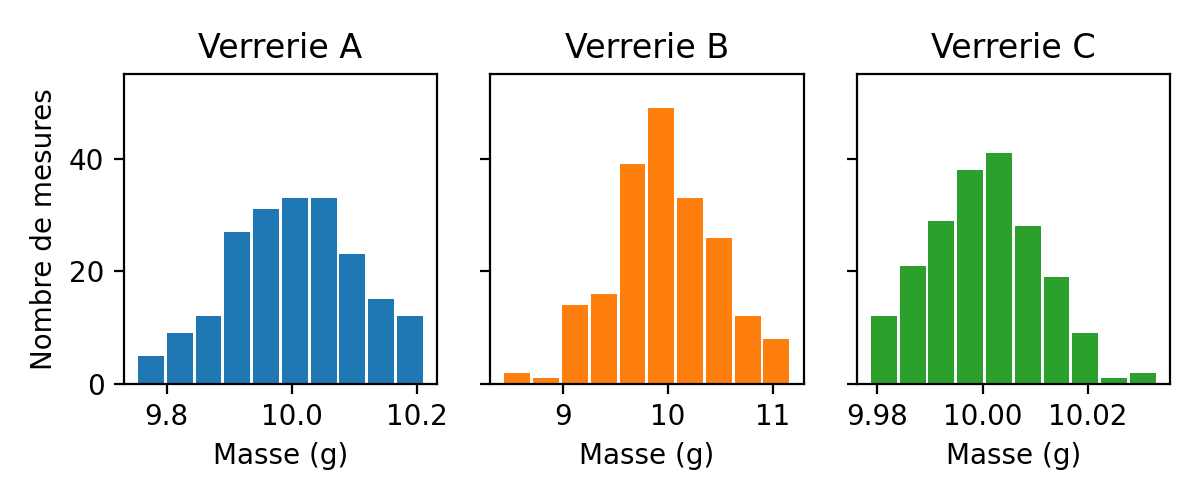
\includegraphics[scale=1]{../images/precision_verrerie.png}
\end{figure}
\begin{enumerate}[resume]
\item \emph{Question facultative:} En traçant l'allure de chaque histogramme comme une courbe en forme de cloche, représenter à main levée sur un même schéma les trois histogrammes A, B et C.
\item À quelle verrerie correspondent les données de l'histogramme \og Verrerie C \fg{} ?
Celles de l'histogramme \og Verrerie B \fg{} ?
Celles de l'histogramme \og Verrerie A \fg{} ?
Justifier.
\end{enumerate}

\section{Encore un peu d'eau salée}

On souhaite réaliser \unit{50}{mL} d'eau salée à la concentration massique $C_\mathrm{m} = \unit{150}{g/L}$.
On dispose de sel, d'eau et de tout le matériel nécessaire.
\begin{enumerate}[resume]
\item Déterminer la masse de sel à peser.
La formule littérale est attendue, ainsi que le détail des conversions.
\item Donner la liste du matériel nécessaire pour la manipulation.
\item Donner les différentes étapes de manipulation sous la forme de schémas.
\item Comment s'appelle la manipulation réalisée pour préparer cette solution.
\end{enumerate}

Après avoir préparé la solution, on la pèse (sans la verrerie utilisée pour la préparer) : les \unit{50}{mL} de solution ont une masse $m=\unit{54{,}9}{g}$.
\begin{enumerate}[resume]
\item Calculer la masse volumique $\rho$ de la solution, exprimée en kilogramme par litre.
La formule littérale est attendue, ainsi que le détail des conversions.
\item Quelle serait la valeur de la masse volumique $\rho$ si la concentration massique de la solution était $C_\mathrm{m} = \unit{0}{g/L}$ ?
Expliquer pourquoi.
\item Les valeurs de masse volumique pour des solutions de concentration massique $C_\mathrm{m} = \unit{0}{g/L}$ et $C_\mathrm{m} = \unit{150}{g/L}$ des questions précédentes sont-elles en accord avec la courbe ci-dessous.
Justifier.
\item En moyenne, l'eau de la mer Morte a une masse volumique $\rho = \unit{1{,175}}{kg/L}$.
En vous aidant de la courbe, en déduire sa concentration massique en sel.
Quelle est alors la masse de sel dans 1 Litre de mer Morte ?
\item Proposer une autre méthode permettant de déterminer la masse de sel présente dans \unit{1}{L} de mer Morte.
\end{enumerate}
\begin{figure}[h]
\center
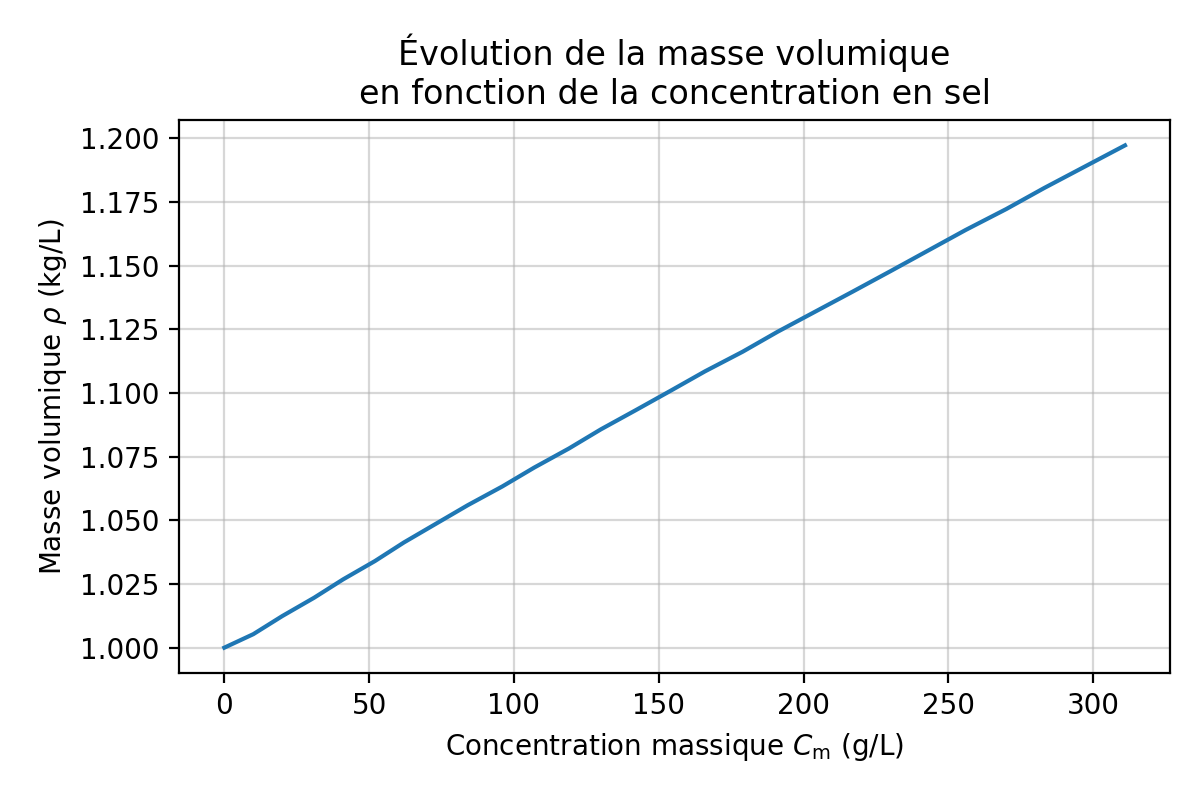
\includegraphics[scale=1]{../images/densite_saumure.png}
\end{figure}

\begin{enumerate}[resume]
\item Cette courbe ne peut être tracée que jusqu'à une valeur de concentration massique de \unit{358{,}5}{g/L}.
À votre avis, pourquoi est-il impossible d'aller plus loin ?
\end{enumerate}

\end{document}